\documentclass[10pt]{standalone}
\usepackage[utf8]{inputenc}
\usepackage{helvet}
\usepackage{amsmath}
\renewcommand{\familydefault}{\sfdefault}
\usepackage{tikz}
\usetikzlibrary{arrows.meta, positioning, fit, calc, shapes.geometric, decorations.pathreplacing, backgrounds}

\definecolor{emeraldpine}{HTML}{1A4D3E}
\definecolor{harvardcrimson}{HTML}{A51C30}
\definecolor{ethdarkblue}{HTML}{1F407A}
\definecolor{ethpetrol}{HTML}{007A87}
\definecolor{ethbronze}{HTML}{B87333}
\definecolor{ethpurple}{HTML}{5B4B8A}
\definecolor{ink}{HTML}{1A202C}
\definecolor{softink}{HTML}{4A5568}
\definecolor{paleink}{HTML}{A0AEC0}
\definecolor{cardbg}{HTML}{F8FAFC}
\definecolor{shadecolor}{HTML}{F4F6F9}

\begin{document}
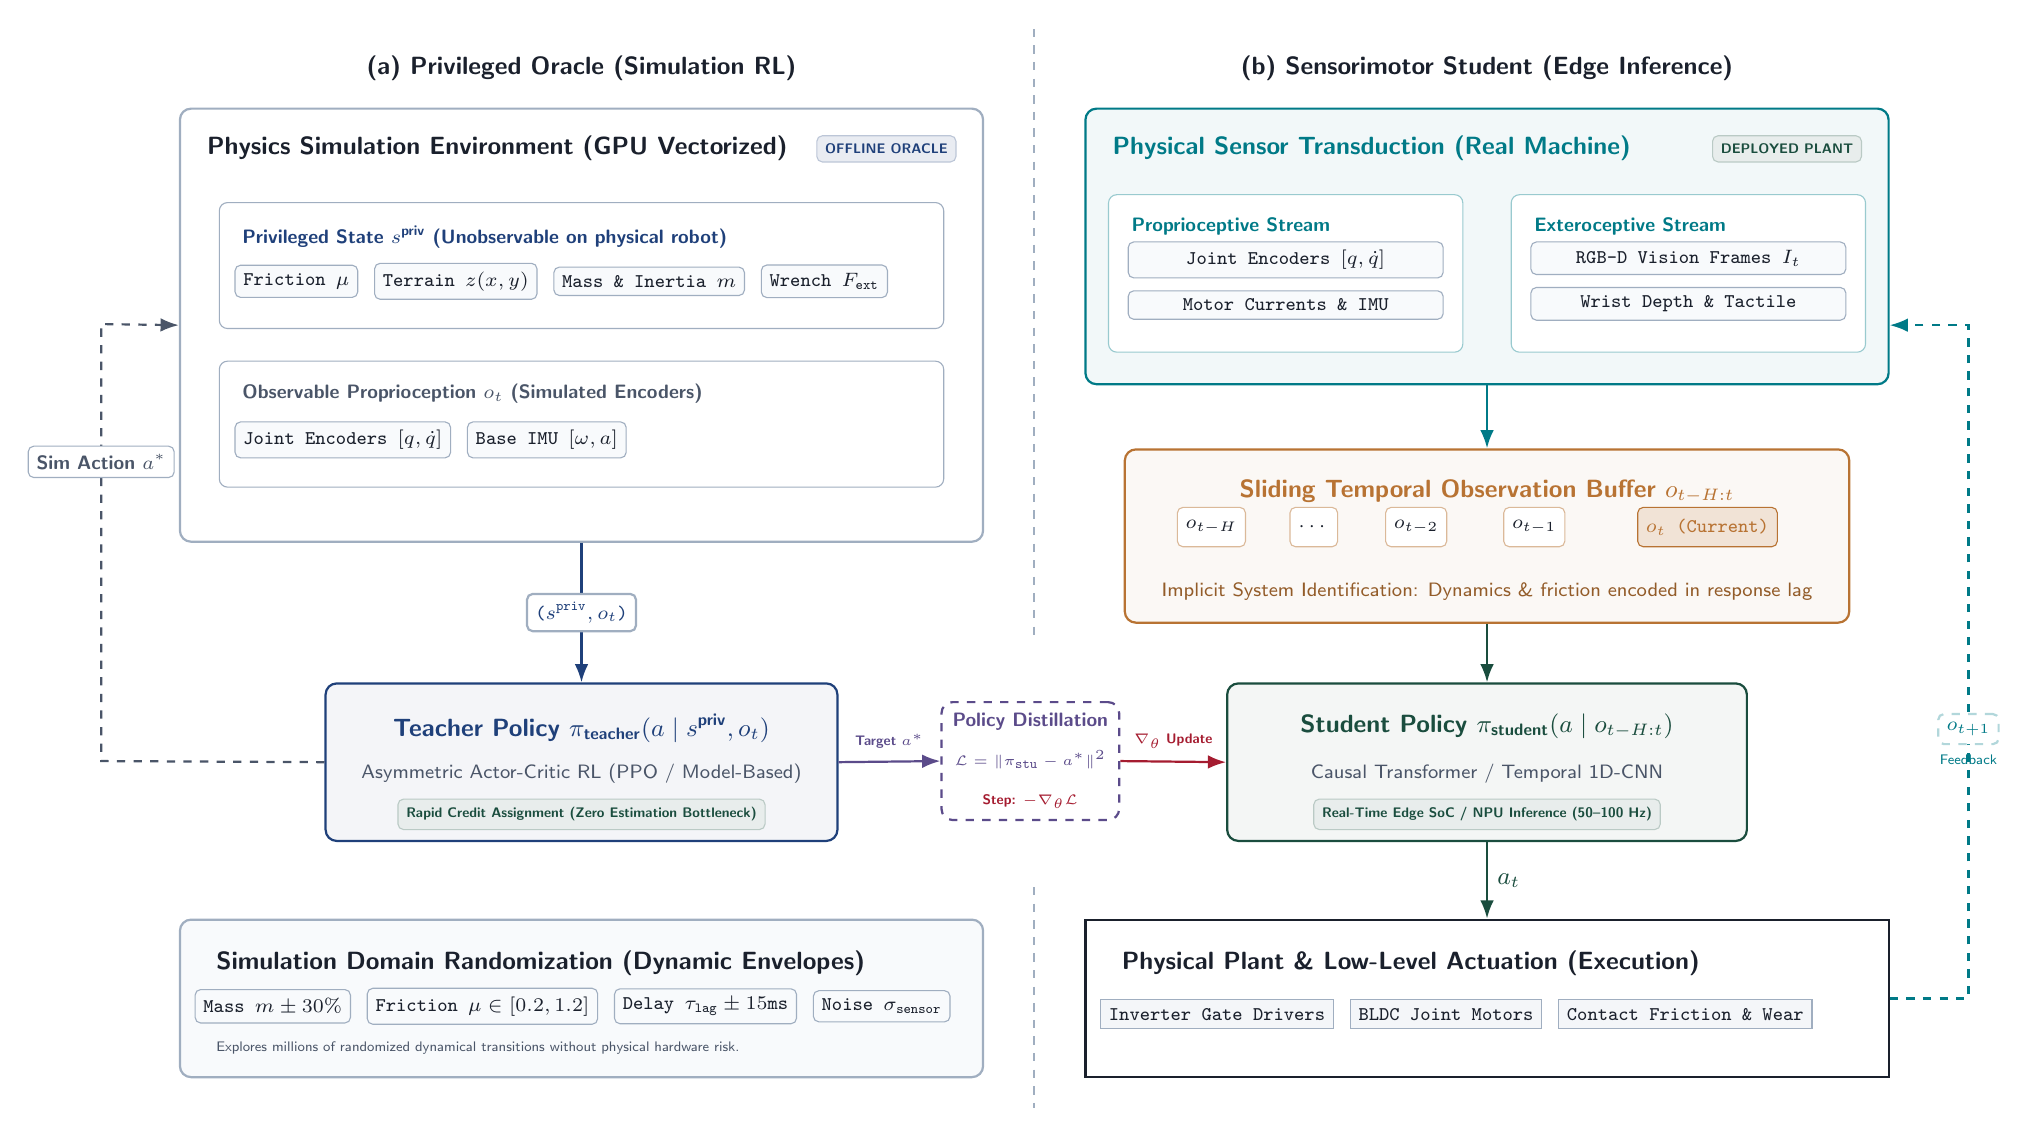
\begin{tikzpicture}[
    >=Latex,
    font=\sffamily,
    title/.style={font=\bfseries\small, text=ink},
    subtitle/.style={font=\scriptsize, text=softink},
    chip/.style={draw, paleink, fill=cardbg, rounded corners=2pt, font=\scriptsize\ttfamily, inner sep=3pt, text=ink},
    subbox/.style={draw, paleink, rounded corners=3pt, fill=white, inner sep=5pt},
]

% Divider (interrupted around distillation bridge)
\draw[paleink, thick, dashed] (5.75, 0.5) -- (5.75, -7.2);
\draw[paleink, thick, dashed] (5.75, -10.4) -- (5.75, -13.2);

% -------------------------------------------------------------
% Left Panel: Privileged Oracle
% -------------------------------------------------------------
\node[title] (left_title) at (0, 0) {(a) Privileged Oracle (Simulation RL)};

% Physics Simulator Background
\node[draw, paleink, thick, rounded corners=4pt, fill=white, minimum width=10.2cm, minimum height=5.5cm, anchor=north] (sim_bg) at (0, -0.5) {};

% Simulator Header
\node[anchor=north west, font=\small\bfseries, text=ink, inner sep=10pt] (sim_title) at (sim_bg.north west) {Physics Simulation Environment (GPU Vectorized)};
\node[anchor=north east, chip, fill=ethdarkblue!10, draw=ethdarkblue!30, text=ethdarkblue, font=\tiny\bfseries, xshift=-10pt, yshift=-10pt] at (sim_bg.north east) {OFFLINE ORACLE};

% Privileged State Subbox
\node[draw, paleink, rounded corners=3pt, fill=white, minimum width=9.2cm, minimum height=1.6cm, anchor=north] (priv_box) at ($(sim_bg.north)+(0, -1.2)$) {};
\node[anchor=north west, font=\scriptsize\bfseries, text=ethdarkblue, xshift=5pt, yshift=-5pt] at (priv_box.north west) {Privileged State $s^{\text{priv}}$ (Unobservable on physical robot)};

% Chips inside Privileged State
\node[chip, anchor=west] (chip_mu) at ($(priv_box.west)+(0.2, -0.2)$) {Friction $\mu$};
\node[chip, anchor=west] (chip_terrain) at ($(chip_mu.east)+(0.2, 0)$) {Terrain $z(x,y)$};
\node[chip, anchor=west] (chip_mass) at ($(chip_terrain.east)+(0.2, 0)$) {Mass \& Inertia $m$};
\node[chip, anchor=west] (chip_wrench) at ($(chip_mass.east)+(0.2, 0)$) {Wrench $F_{\text{ext}}$};

% Observable Proprioception Subbox
\node[draw, paleink, rounded corners=3pt, fill=white, minimum width=9.2cm, minimum height=1.6cm, anchor=north] (obs_box) at ($(priv_box.south)+(0, -0.4)$) {};
\node[anchor=north west, font=\scriptsize\bfseries, text=softink, xshift=5pt, yshift=-5pt] at (obs_box.north west) {Observable Proprioception $o_t$ (Simulated Encoders)};

% Chips inside Observable Proprioception
\node[chip, anchor=west] (chip_enc) at ($(obs_box.west)+(0.2, -0.2)$) {Joint Encoders $[q, \dot{q}]$};
\node[chip, anchor=west] (chip_imu) at ($(chip_enc.east)+(0.2, 0)$) {Base IMU $[\omega, a]$};

% Teacher Policy (aligned vertically with Student Policy at y = -7.8)
\node[draw, ethdarkblue, thick, rounded corners=4pt, fill=ethdarkblue!5, minimum width=6.5cm, minimum height=2.0cm, anchor=north] (teacher_bg) at (0, -7.8) {};
\node[anchor=north, font=\small\bfseries, text=ethdarkblue, yshift=-8pt] (teacher_title) at (teacher_bg.north) {Teacher Policy $\pi_{\text{teacher}}(a \mid s^{\text{priv}}, o_t)$};
\node[anchor=north, subtitle, yshift=-26pt] at (teacher_bg.north) {Asymmetric Actor-Critic RL (PPO / Model-Based)};
\node[anchor=north, chip, fill=emeraldpine!10, draw=emeraldpine!30, text=emeraldpine, font=\tiny\bfseries, yshift=-42pt] at (teacher_bg.north) {Rapid Credit Assignment (Zero Estimation Bottleneck)};

% Arrow Sim -> Teacher
\draw[->, ethdarkblue, thick] (sim_bg.south) -- (teacher_bg.north) node[midway, fill=white, draw=paleink, rounded corners=2pt, inner sep=3pt, font=\scriptsize\ttfamily, text=ethdarkblue] {($s^{\text{priv}}, o_t$)};

% Feedback Arrow from Teacher -> Simulator (routed cleanly outside sim_bg)
\draw[->, softink, thick, dashed] (teacher_bg.west) -- (-6.1, -8.8) -- (-6.1, -3.25) -- (sim_bg.west);
\node[fill=white, draw=paleink, rounded corners=2pt, inner sep=3pt, font=\scriptsize\bfseries, text=softink] at (-6.1, -5.0) {Sim Action $a^*$};

% Domain Randomization (aligned with Physical Plant at y = -10.8)
\node[draw, paleink, thick, rounded corners=4pt, fill=cardbg, minimum width=10.2cm, minimum height=2.0cm, anchor=north] (dr_bg) at (0, -10.8) {};
\node[anchor=north west, font=\small\bfseries, text=ink, xshift=10pt, yshift=-8pt] at (dr_bg.north west) {Simulation Domain Randomization (Dynamic Envelopes)};

\node[chip, anchor=west] (dr_mass) at ($(dr_bg.west)+(0.2, -0.1)$) {Mass $m \pm 30\%$};
\node[chip, anchor=west] (dr_fric) at ($(dr_mass.east)+(0.2, 0)$) {Friction $\mu \in [0.2, 1.2]$};
\node[chip, anchor=west] (dr_delay) at ($(dr_fric.east)+(0.2, 0)$) {Delay $\tau_{\text{lag}} \pm 15\text{ms}$};
\node[chip, anchor=west] (dr_noise) at ($(dr_delay.east)+(0.2, 0)$) {Noise $\sigma_{\text{sensor}}$};

\node[anchor=south west, font=\tiny, text=softink, xshift=10pt, yshift=5pt] at (dr_bg.south west) {Explores millions of randomized dynamical transitions without physical hardware risk.};

% -------------------------------------------------------------
% Right Panel: Sensorimotor Student
% -------------------------------------------------------------
\node[title] (right_title) at (11.5, 0) {(b) Sensorimotor Student (Edge Inference)};

% Physical Sensor Transduction Background
\node[draw, ethpetrol, thick, rounded corners=4pt, fill=ethpetrol!5, minimum width=10.2cm, minimum height=3.5cm, anchor=north] (sensor_bg) at (11.5, -0.5) {};

% Sensor Header
\node[anchor=north west, font=\small\bfseries, text=ethpetrol, inner sep=10pt] at (sensor_bg.north west) {Physical Sensor Transduction (Real Machine)};
\node[anchor=north east, chip, fill=emeraldpine!10, draw=emeraldpine!30, text=emeraldpine, font=\tiny\bfseries, xshift=-10pt, yshift=-10pt] at (sensor_bg.north east) {DEPLOYED PLANT};

% Proprioceptive Stream Subbox
\node[draw, ethpetrol!40, rounded corners=3pt, fill=white, minimum width=4.5cm, minimum height=2cm, anchor=north west] (prop_box) at ($(sensor_bg.north west)+(0.3, -1.1)$) {};
\node[anchor=north west, font=\scriptsize\bfseries, text=ethpetrol, xshift=5pt, yshift=-5pt] at (prop_box.north west) {Proprioceptive Stream};
\node[chip, anchor=north, minimum width=4.0cm, fill=cardbg] (r_enc) at ($(prop_box.north)+(0, -0.6)$) {Joint Encoders $[q, \dot{q}]$};
\node[chip, anchor=north, minimum width=4.0cm, fill=cardbg] (r_curr) at ($(r_enc.south)+(0, -0.15)$) {Motor Currents \& IMU};

% Exteroceptive Stream Subbox
\node[draw, ethpetrol!40, rounded corners=3pt, fill=white, minimum width=4.5cm, minimum height=2cm, anchor=north east] (ext_box) at ($(sensor_bg.north east)+(-0.3, -1.1)$) {};
\node[anchor=north west, font=\scriptsize\bfseries, text=ethpetrol, xshift=5pt, yshift=-5pt] at (ext_box.north west) {Exteroceptive Stream};
\node[chip, anchor=north, minimum width=4.0cm, fill=cardbg] (r_rgbd) at ($(ext_box.north)+(0, -0.6)$) {RGB-D Vision Frames $I_t$};
\node[chip, anchor=north, minimum width=4.0cm, fill=cardbg] (r_tact) at ($(r_rgbd.south)+(0, -0.15)$) {Wrist Depth \& Tactile};

% Observation Buffer
\node[draw, ethbronze, thick, rounded corners=4pt, fill=ethbronze!5, minimum width=9.2cm, minimum height=2.2cm, anchor=north] (buffer_bg) at ($(sensor_bg.south)+(0, -0.8)$) {};
\node[anchor=north, font=\small\bfseries, text=ethbronze, yshift=-8pt] at (buffer_bg.north) {Sliding Temporal Observation Buffer $o_{t-H:t}$};

\begin{scope}[shift={($(buffer_bg.north)+(-4.0, -1.0)$)}]
    \node[chip, draw=ethbronze!50, fill=white, minimum height=0.5cm] at (0.5,0) {$o_{t-H}$};
    \node[chip, draw=ethbronze!50, fill=white, minimum height=0.5cm] at (1.8,0) {$\cdots$};
    \node[chip, draw=ethbronze!50, fill=white, minimum height=0.5cm] at (3.1,0) {$o_{t-2}$};
    \node[chip, draw=ethbronze!50, fill=white, minimum height=0.5cm] at (4.6,0) {$o_{t-1}$};
    \node[chip, draw=ethbronze, fill=ethbronze!20, font=\scriptsize\ttfamily\bfseries, text=ethbronze, minimum height=0.5cm] at (6.8,0) {$o_t$ (Current)};
\end{scope}
\node[anchor=south, font=\scriptsize, text=ethbronze!80!black, yshift=5pt] at (buffer_bg.south) {Implicit System Identification: Dynamics \& friction encoded in response lag};

\draw[->, ethpetrol, thick] (sensor_bg.south) -- (buffer_bg.north);

% Student Policy (aligned vertically with Teacher Policy at y = -7.8)
\node[draw, emeraldpine, thick, rounded corners=4pt, fill=emeraldpine!5, minimum width=6.6cm, minimum height=2.0cm, anchor=north] (student_bg) at (11.5, -7.8) {};
\node[anchor=north, font=\small\bfseries, text=emeraldpine, yshift=-8pt] at (student_bg.north) {Student Policy $\pi_{\text{student}}(a \mid o_{t-H:t})$};
\node[anchor=north, subtitle, yshift=-26pt] at (student_bg.north) {Causal Transformer / Temporal 1D-CNN};
\node[anchor=north, chip, fill=emeraldpine!10, draw=emeraldpine!30, text=emeraldpine, font=\tiny\bfseries, yshift=-42pt] at (student_bg.north) {Real-Time Edge SoC / NPU Inference (50--100 Hz)};

\draw[->, emeraldpine, thick] (buffer_bg.south) -- (student_bg.north);

% Physical Plant (aligned vertically with Domain Randomization at y = -10.8)
\node[draw, ink, thick, fill=white, minimum width=10.2cm, minimum height=2.0cm, anchor=north, rounded corners=0] (plant_bg) at (11.5, -10.8) {};
\node[anchor=north west, font=\small\bfseries, text=ink, xshift=10pt, yshift=-8pt] at (plant_bg.north west) {Physical Plant \& Low-Level Actuation (Execution)};

\node[chip, anchor=west, rounded corners=0, fill=shadecolor] (p_inv) at ($(plant_bg.west)+(0.2, -0.2)$) {Inverter Gate Drivers};
\node[chip, anchor=west, rounded corners=0, fill=shadecolor] (p_bldc) at ($(p_inv.east)+(0.2, 0)$) {BLDC Joint Motors};
\node[chip, anchor=west, rounded corners=0, fill=shadecolor] (p_wear) at ($(p_bldc.east)+(0.2, 0)$) {Contact Friction \& Wear};

\draw[->, emeraldpine, thick] (student_bg.south) -- (plant_bg.north) node[midway, right, font=\small\ttfamily\bfseries, text=emeraldpine] {$a_t$};

% Physical Loop
\draw[->, ethpetrol, thick, dashed] (plant_bg.east) -- ++(1.0, 0) |- ($(sensor_bg.east)+(0, -1.0)$) node[pos=0.2, fill=white, draw=ethpetrol!30, rounded corners=2pt, inner sep=3pt, font=\scriptsize\ttfamily\bfseries, text=ethpetrol] {$o_{t+1}$} node[pos=0.2, below=0.2cm, font=\tiny, text=ethpetrol] {Feedback};

% -------------------------------------------------------------
% Distillation Bridge with Explicit Loss and Gradient Flow
% -------------------------------------------------------------
\node[fill=white, draw=ethpurple, thick, dashed, rounded corners=4pt, inner sep=4pt, align=center] (distill_box) at (5.7, -8.8) {
    \textbf{\textcolor{ethpurple}{\scriptsize Policy Distillation}}\\[2pt]
    \textcolor{ethpurple}{\tiny\ttfamily $\mathcal{L} = \|\pi_{\text{stu}} - a^*\|^2$}\\[2pt]
    \textcolor{harvardcrimson}{\tiny\bfseries Step: $-\nabla_\theta \mathcal{L}$}
};

% Teacher target action -> Distillation Loss
\draw[->, ethpurple, thick] (teacher_bg.east) -- (distill_box.west) node[midway, above=1pt, font=\tiny\bfseries, text=ethpurple] {Target $a^*$};

% Distillation loss gradient update -> Student Policy
\draw[->, harvardcrimson, thick] (distill_box.east) -- (student_bg.west) node[midway, above=1pt, font=\tiny\bfseries, text=harvardcrimson] {$\nabla_\theta$ Update};

\end{tikzpicture}
\end{document}
